\documentclass[11pt,letterpaper]{report}

\author{Mendoza-Cortes Group}
\title{Machine Learning Methods in Sciences}
\usepackage{fancyhdr}
%\lhead{Report}
\rhead{Mendoza-Cortes Group}
%\rhead{\today}
\headheight 35pt 

%%%%%%%%%%%%%%%%%%%%%%%%%%%%%%%%%%%%
% Begin Load Packages %%%%%%%%%%%%%%%%%%%%%%%%
%%%%%%%%%%%%%%%%%%%%%%%%%%%%%%%%%%%%

\usepackage{listings}
\usepackage{etex}
\usepackage{graphicx}
\usepackage{booktabs}
%\usepackage[flushleft]{threeparttable}
\usepackage[margin=1.0in]{geometry}
\usepackage{caption}
\usepackage{subcaption}
%\usepackage{titlesec}
\usepackage{hyperref}
\usepackage{url}
\hypersetup{colorlinks=true,  % false: boxed links; true: colored links
	linkcolor=blue,   % color of internal links
	urlcolor=magenta, % color of external links
	citecolor=blue    % color of links to bibliography
}

% Package for chemistry formulas %%%%%%%%%%%%%%%%%%%%%%%%
\usepackage[version=3]{mhchem}

%%%%%%%%%%%%%%%%%%%%%%%%%%%%%%%%%%%%
% End Load Packages %%%%%%%%%%%%%%%%%%%%%%%%%
%%%%%%%%%%%%%%%%%%%%%%%%%%%%%%%%%%%%


%%%%%%%%%%%%%%%%%%%%%%%%%%%%%%%%%%%%
% Begin Extra Functionality %%%%%%%%%%%%%%%%%%%%%%
%%%%%%%%%%%%%%%%%%%%%%%%%%%%%%%%%%%%
% Adjust sticky notes
\usepackage{xargs} 
\usepackage[colorinlistoftodos,prependcaption,textsize=tiny]{todonotes}
\newcommandx{\you}[2][1=]{\todo[linecolor=green,backgroundcolor=green!25,bordercolor=green,#1]{#2}}
\newcommandx{\jose}[2][1=]{\todo[linecolor=red,backgroundcolor=red!25,bordercolor=red,#1]{#2}}
\newcommandx{\both}[2][1=]{\todo[linecolor=blue,backgroundcolor=blue!25,bordercolor=blue,#1]{#2}}
%%%%%%%%%%%%%%%%%%%%%%%%%%%%%%%%%%%%
% End Extra Functionality %%%%%%%%%%%%%%%%%%%%%%%
%%%%%%%%%%%%%%%%%%%%%%%%%%%%%%%%%%%%


%%%%%%%%%%%%%%%%%%%%%%%%%%%%%%%%%%%%
%Begin Table of contents extras. This will put the title Page on top of the table of contents
%%%%%%%%%%%%%%%%%%%%%%%%%%%%%%%%%%%%
\addtocontents{toc}{~\hfill\textbf{\large Page}\par}
\addtocontents{lof}{~\hfill\textbf{\large Page}\par}
\addtocontents{lot}{~\hfill\textbf{\large Page}\par}
%\addcontentsline{toc}{section}{Title}
%%%%%%%%%%%%%%%%%%%%%%%%%%%%%%%%%%%%
% End Table of contents extras
%%%%%%%%%%%%%%%%%%%%%%%%%%%%%%%%%%%%



%%%%%%%%%%%%%%%%%%%%%%%%%%%%%%%%%%%%
% Begin the Actual Document %%%%%%%%%%%%%%%%%%%%%
%%%%%%%%%%%%%%%%%%%%%%%%%%%%%%%%%%%%


\begin{document}
	
	\setcounter{page}{1}
	\pagenumbering{roman}
	\thispagestyle{empty}
	
	
	
	
	\maketitle
	
	\clearpage
	\newpage
	\pagenumbering{arabic}
	\setcounter{page}{1}
	\pagestyle{fancy}
	
	%*************************************************************** %
	% % % % % % % % % % % % % % % % % % % % % % % % % % % % % % % % %
	%*************************************************************** %
	%*************************************************************** %
	% % % % % % % % % % % % % % % % % % % % % % % % % % % % % % % % %
	%*************************************************************** %
	%*************************************************************** %
	% % % % % % % % % % % % % % % % % % % % % % % % % % % % % % % % %
	%*************************************************************** %
	
	%%%%%%%%%%%%%%%%%%%%%%%%%%%%%%%%%%%%
	% Begin Chapter Document %%%%%%%%%%%%%%%%%%%%%
	%%%%%%%%%%%%%%%%%%%%%%%%%%%%%%%%%%%%
	
	
	\begin{abstract}
		The following guide is intended for non CS majors that would like to use  Machine Learning on their field. It contains applications to Art, Engineering, Physics, Medicine and Chemistry.
	\end{abstract}
	
	\clearpage
	\newpage
	\section{Motivation}
		Which machine learning algorithms should you use for your research or project? There are already several automatized programs  that take your data and evaluate machine learning algorithms on it. By design, those methods won't use the optimal parameters or don't use the recent technology. In this notes we aim to give several examples of algorithms and applications to help you identify the method most suitable for your problem while understanding how to use the more capabilities of the algorithm. This will be an important difference if you are interested in research, or to optimize a solution to a problem. In case that all you want is a quick solution without worrying if it is optimal or not, you may prefer to use automatized methods instead, we will mention a couple of them in the corresponding section. 
		
		Our goal is to make this notes accessible for non CS majors with plenty of examples that will help you identify if your particular problem can be solve with the method.
	
	Software required:
	This guide will require a basic knowledge of python 3, we recommend to install it with Anaconda. We also have notebooks that serve as an introduction to Python.
	Half of the lectures use  Sklearn \cite{Pedregosa2011}, the section on Neural Networks contains a lecture on Keras\cite{chollet2015keras}. For the advanced parts we have lectures on Pytorch\cite{paszke2017automatic} and  Tensorflow\cite{tensorflow2015-whitepaper}.
	
	
	
	%%*************************************************************** %
	%% % % % % % % % % % % % % % % % % % % % % % % % % % % % % % % % %
	%%*************************************************************** %
	%%*************************************************************** %
	%% % % % % % % % % % % % % % % % % % % % % % % % % % % % % % % % %
	%%*************************************************************** %
	%%*************************************************************** %
	%% % % % % % % % % % % % % % % % % % % % % % % % % % % % % % % % %
	%%*************************************************************** %
	%
	%%%%%%%%%%%%%%%%%%%%%%%%%%%%%%%%%%%%%
	%% Begin Chapter Document %%%%%%%%%%%%%%%%%%%%%
	%%%%%%%%%%%%%%%%%%%%%%%%%%%%%%%%%%%%%
    \subsection{Fairness}
	For motivational purposes assume that you have measured data, and for each value you have a label. Perhaps you have a list of characteristics of breast cancer samples and the label is 1 if the cancer is malignant or 0 if it is benign as in \href{https://scikit-learn.org/stable/datasets/index.html#breast-cancer-dataset}{Breast cancer Wisconsin (diagnostic) dataset}\cite{wcancer}, another example is the data of police misconduct in Chicago and the labels are the officer's race as in \href{https://data.cpdp.co/data/L5rG3q/}{Citizens Police Data Project}\cite{wpolice}. The main task for us is to find if we can we make reasonable predictions for the labels of new, unseen, data values.

    The algorithm will return a class based on the algorithm's design and training. Which data do we use for training it and what we do with the output are choices made by humans and this will have consequences. We recommend to take the 70 min \href{https://developers.google.com/machine-learning/crash-course/fairness/video-lecture?utm_source=keyword-blog&utm_medium=blog&utm_campaign=mle-outreach&utm_term=&utm_content=mlcc-fairness}{Fairness training}\cite{wfair} to prevent different types of bias on your project. 

	\subsection{Preprocessing Data}

	
	 A big part of the performance of a machine learning algorithm relies on preprocessing the data. If we don't have enough data, or if it is biased, the algorithms will reflect those deficiencies in the output. For example, for the contest and 	 \href{	  http://agile-iot.eu/adaptation/}{art event Adaptation}\cite{wadaptation} we 
	 \href{	 https://www.sciartmagazine.com/straight-talk-justus-harris.html}{ worked with 3D-scanners}\cite{wexhibition} 
	  until we realized they failed with people of color. The community on twitter suggested that it was an illumination issue, we claim that deciding that the algorithm is ready after testing it only on white people while not caring about the results on people of color is a choice that makes the algorithm biased. After all, that scanner was used on toys and the toy producer was not expecting kids to have special illumination while using the toys.
	 
	 An important lesson here is that \href{ https://www.quora.com/In-machine-learning-is-more-data-always-better-than-better-algorithms}{data quality}\cite{wdata} is a priority. 
	 Since data is collected by humans, you should always look for mistakes by cleaning the data. The  notebook `` First Machine Learning Notebook'' is an excellent guide on data analysis followed by ``Higher Dimensions'' which explains the curse of dimensionality and gives an introduction to higher dimensional geometry. 
	  
	  % As preprocessing we consider the problem of finding a good representation of our data that helps with the classification process. We will use Taylor series to Build such a map, we know that for a convex function the Hessian is positive definite. So one strategy would be to add any positive definite quadratic form as the non linear part of our map, in ``Information Geometry and Dynamic Entropy'' we review the implications of this process for information theory.
	  %
 	\section{Machine Learning algorithms covered}
 	
 	
 	
	\subsection{SVC}
	Imagine that you are designing a new material. First you create it in vitro, and then you have a team that will materialize those designs. The task is to determine when something goes wrong before investing in the realization of the material; it is fairly easy to determine what are good properties but it is a complex task to imagine what could be bad specially on a multi scale process, perhaps the atomic configuration is unstable, the material is below quality, or there is a similar  material in properties and quality  with a lower price.  Since collection of example data of a faulty system  can be expensive, or just impossible,  there is no way to describe a priory all the possible defects on the material. SVM can be use to attack this kind of problems as explained in the notebooks ``Support Vector Machine".
	
	The general idea is explained as follows:
	\begin{figure}[h!]
		\centering
		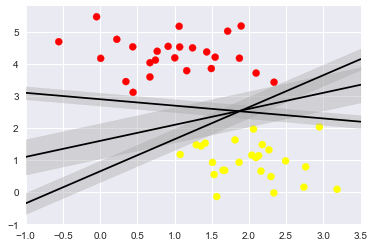
\includegraphics[width=0.45\linewidth]{figures/svcl.png}
		\caption{}
		\label{fig:lines}
	\end{figure} 
	
	Assume we are dealing with classification of labeled data. We have data with information about in which class do they belong. We want an algorithm to classify new unseen data. In good cases it is possible to use lines to separate classes and then the question becomes, among all possible lines, which one is best to use? as in fig \ref{fig:lines}. Once we have decided how to evaluate quality, we will be able to select a line. A natural requirement is that the algorithm should be robust to new data and minimize the number of miss classifications. In the notebook ``SVM'' you can see how the algorithm SVC looks for  the coefficients of such a line.

\begin{figure}[h!]
	\centering
	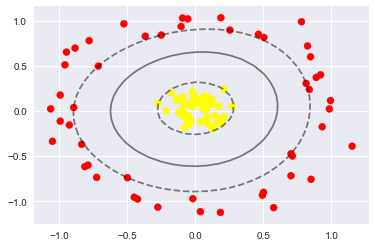
\includegraphics[width=0.45\linewidth]{figures/svc.png}
	\caption{}
	\label{fig:kernel}
\end{figure} 
	
 Most real life cases are not linearly separable, but sometimes we can transform the features hoping that the new features can be separated  with hyper planes. On the image \ref{fig:kernel} we add a third coordinate to the data, the distance to the origin. Then in $R^3$ it is easy to find a plane $z=.6$ that classifies our data. SVM performs better if we pre-process the data following the rules on the notebook ``Cleaning data''. 
 
How can we use this algorithm to find anomalies in new products? we can assume that good products have label 1 and products that are outliers have label 0. By training the SVC this way, it will learn to classify products in regular or outliers. It will recognize when a new product is far from the standard as in fig \ref{fig:novelty}. This idea is explained in the notebook ``SVC II''. 
	
	\begin{figure}[h!]
		\centering
		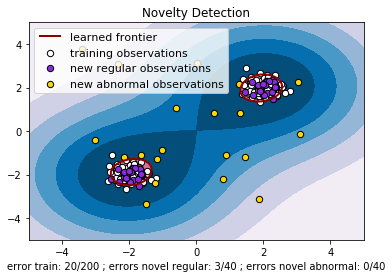
\includegraphics[width=0.45\linewidth]{figures/novelty.png}
		\caption{}
		\label{fig:novelty}
	\end{figure} 
	
% Needed:	Brief description of good and bad points of SVM 
	\subsection{Neural Networks}  
	
	We saw that SVM uses  hyperplanes to separate the data, and that sometimes a transformation of the data is needed. In feed forward neural networks we use iterations of non linear functions followed by matrix transformations that transforms the data to create a classification.
	
	 A neural network is a composition of  functions of the form:
	$x\rightarrow \sigma(W\cdot x+b)$ where $x,b,$ are vectors, $W$ is a matrix, and $\sigma$ stands for a non linear function applied entry wise to the coordinates of the vector  $W\cdot x+b$.
	It is standard notation to represent matrices  $W$ as arrows from the domain of $x$ to the domain of $w\cdot x + b$ as in \ref{fig:nn}. For details see the notebook 'Neural Network'.
	 Finding the coefficients of those matrices requires multivariable calculus and the chain rule. In ``Neural Networks'' you can find an introduction to Keras, which we consider the most friendly language to use Neural Networks, and a deeper explanation of how Neural Networks work and can be trained.	
	
	
	An application of Neural Networks to chemistry is contained in the note ``Poterntial Energy Surface ANN'' where we describe the work of The Roitberg group in University of Florida, a transferable deep learning potential: ANAKIN-ME (Accurate NeurAl networK engINe for Molecular Energies) or ANI for short.
	
    	\begin{figure}[h!]
    	\centering
    	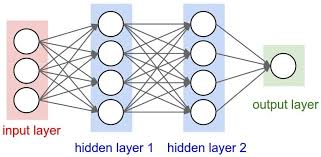
\includegraphics[width=0.45\linewidth]{figures/nn.jpg}
    	\caption{}
    	\label{fig:nn}
    \end{figure} 	
    
    Supposed that you are given  input in different steps, like if the input are letters of a name and you want to predict the nationality of the name. To deal with this kind of data, we need to modify our algorithms. Using time just as another variable will result in classification based on when did the event/measurement happened. But perhaps we want to find a classification based on classifications previous made on the partial data already registered. The lecture ``Recurrent Neural Networks'' deals with networks designed for modeling this sequential data.  
    
    This can be use to make numerical simulations of partial differential equations and ordinary differential equations, and we include an example with pytorch of Character-Level classification of names in ``RNN II''.

	\subsection{CNN}
	
	Given a picture of an Warehouse Shelving, a  neural network can immediately 
	\href{https://developers.google.com/machine-learning/crash-course/fairness/video-lecture?utm_source=keyword-blog&utm_medium=blog&utm_campaign=mle-outreach&utm_term=&utm_content=mlcc-fairness}{identify the objects and restock the items}.
	Chinese government used face recognition to \href{http://fortune.com/2018/10/28/in-china-facial-recognition-tech-is-watching-you/}{identify fugitives in a music concert}.
	
	In order to work with images, we need to solve a problem, images are represented by pixels and a small image has too many pixels. Go to your favorite browser and look for images with exactly  $500\times500$ pixels. That is $250000\times3$ numbers, since we have to select Red Green and Blue for every pixel, and Feed Forward Neural Networks will require you to find multiples of that many coefficients. Besides that, we are not working any more with vectors as the pixels are related with the pixels in their neighborhood.
	
	We need to change the vectors input to matrices input,  and the vectors output to matrix output. You can think of a matrix as a vector with vector entries.  So now the matrices are not only operations but the elements we work on.
	The good thing of image processing is that we have visual help to understand the process. We are going to learn smaller matrices called filters, they may learn geometric concepts as a curve, or a square, see fig \ref{fig:filter}.  
	
	\begin{figure}[h!]
		\centering
		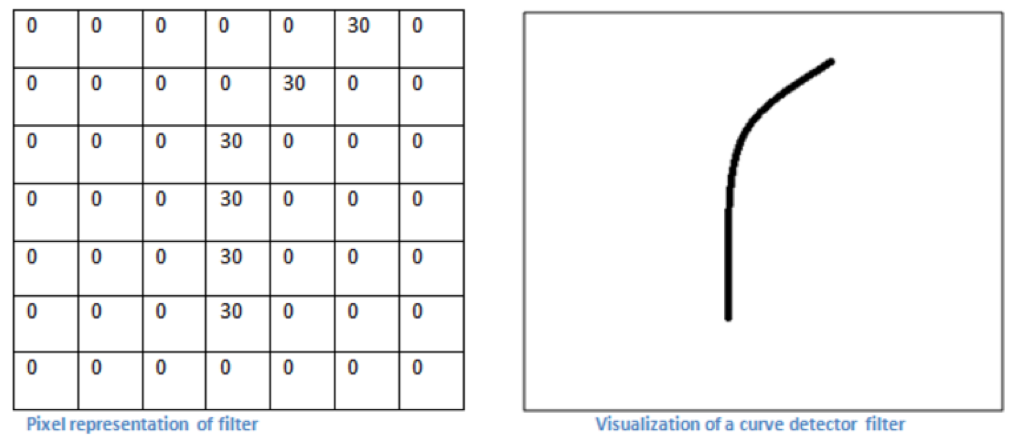
\includegraphics[width=0.45\linewidth]{figures/filter.png}
		\caption{}
		\label{fig:filter}
	\end{figure} 	

    We have a guest post ``CNN'' (in English) from the \href{https://aiacademy.tw}{AI Academy}\cite{wai} where
	 we explain in more detail how CNN work. In lecture ``Deep Dreams" we ask the neural network if it recognizes a pattern on an image and then we modify that image to show the pattern. In `` Style transfer'' we learn images styles and impose them to other images, for example  in \ref{fig:botero} we used a picture of our team and we added the style of a paint of the painter Fernando Botero. %Lecture "L 25" is TBD.
	
	
	\begin{figure}[h!]
		\centering
		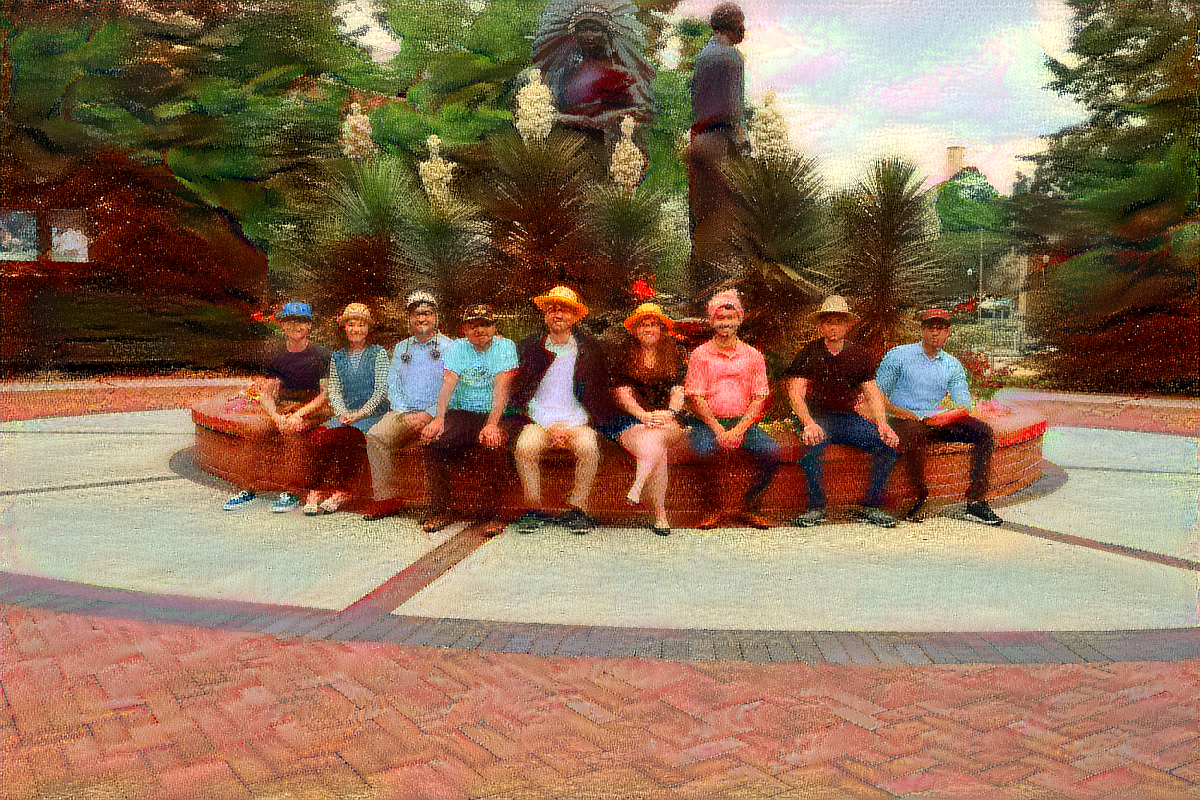
\includegraphics[width=0.45\linewidth]{figures/botero.png}
		\caption{}
		\label{fig:botero}
	\end{figure} 	
	
	
	``Generative Adversarial Networks'' describes a generative method. Suppose that we have a set of examples and we want to generate more images which look like the previous examples. For example, we might have the data set of
	\href{https://github.com/zalandoresearch/fashion-mnist}{fashion-mnist}\cite{wfashion}, a set of  clothes' pictures and we want to generate artificial images as in this \href{https://github.com/spaceLenny/FashionDCGANExample}{ghost wardrobe}\cite{wghost}. While it is hard to train a GAN, it produces interesting results as in this \href{ https://twitter.com/henddkn/status/1067431379804262400?s=19 } {GAN-paint}\cite{wtwitter} or this 
	\href{    https://towardsdatascience.com/password-cracker-generating-passwords-with-recurrent-neural-networks-lstms-9583714a3310 
	}{password cracking}\cite{wpassword} tool.
	
	
	We recommend to read 	\href{    https://arxiv.org/abs/1608.08225 
	}{Why does deep and cheap learning work so well?}\cite{Lin2017}.  The authors use physics to train to explain the way neural networks are capable to make classifications. 
\subsection{Bayesian methods}
In ``Frequentist vs Bayes''
 we introduce Bayesian methods and show how do they differ from the frequetist perspective. 
 
Frequently we want to quantify the accuracy of our predictions. In the ``Markov'' lectures we find a Bayesian approach--one where we consider the values of the parameters as random variables.

Recall Bayes' theorem for training parameters
\begin{equation}
P(\theta|X_{train}, T_{train}) = \frac{P(T_{train}, \theta|X_{train})}{\int P(T_{train}, \theta|X_{train})\;\mathrm{d}\theta} 
\end{equation}

The integral on the bottom is generally not analytic. And for higher dimensional problems, infeasible to calculate. By using Monte Carlo Markov Chain algorithm, it is possible to make estimations.  This is also useful to study   the Ising model, which was created to describe Magnetic and ferromagnetic materials. We also introduce Simulated Annealing and Uncertainty Quantification.
\subsection{SOM}
Self Organizing Maps is a method that allow us to do dimensional reduction. The main idea is to place randomly points and let those points get attracted to the data points, in such a way that clusters will pull the points harder. We expect the points to end up placed in the center of the clusters. We will make this precise on the lecture ``SOM". 
In the following picture we can see an \href{https://github.com/ANNetGPGPU/ANNetGPGPU}{ image
	generated using Self Organizing Maps}\cite{wsom}.

\begin{figure}[h!]
	\centering
	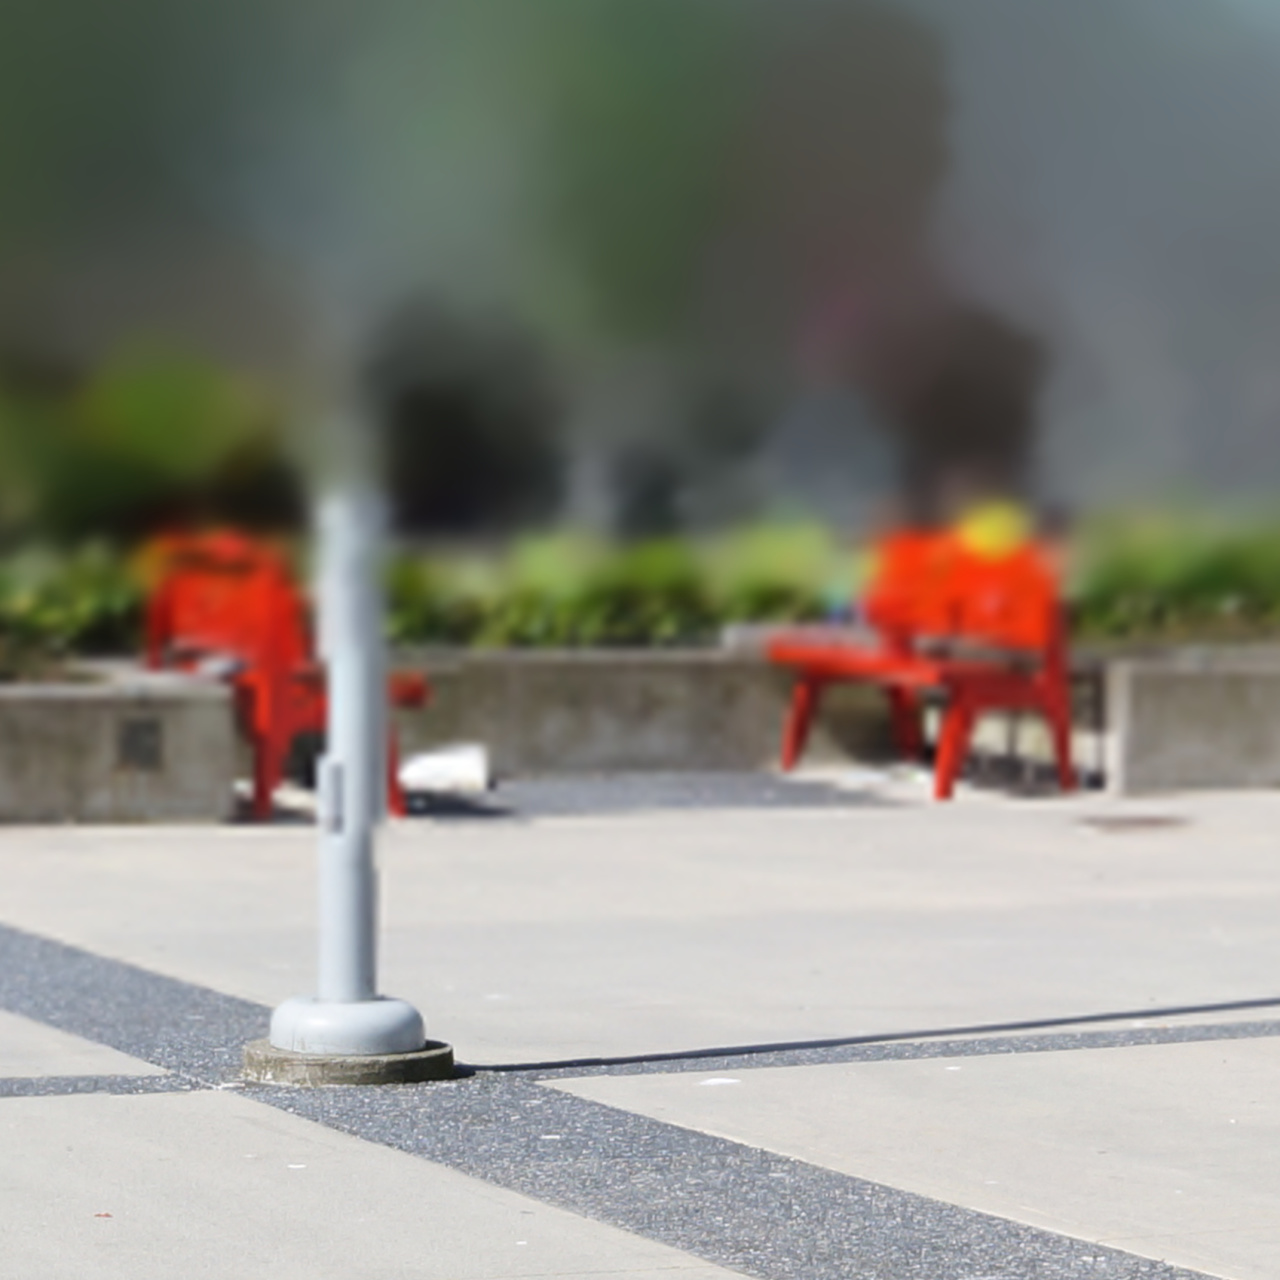
\includegraphics[width=0.45\linewidth]{figures/ex.jpg}
	\caption{SOM image generated.} 
	\label{fig:som}
\end{figure} 	

\subsection{Genetic Algorithms}
A genetic algorithm is a search heuristic  inspired by Charles Darwin’s theory of natural evolution. They reflect the process of natural selection where the fittest individuals are selected for reproduction in order to produce the next generation.



Genetic Algorithms are most commonly used in optimization problems wherein we have to maximize or minimize a given objective function value under a given set of constraints. GAs are also used to characterize various economic models like the cobweb model, game theory equilibrium resolution, asset pricing, etc. They also have been used to plan the path which a robot arm takes by moving from one point to another. We can find more applications in multimodal optimization in which we have to find multiple optimum solutions.



\begin{figure}[h!]
	\centering
	\includegraphics[width=0.45\linewidth]{figures/GAfigure1.png}
	\caption{}
	\label{fig:GA}
\end{figure} 	


Given a problem we define a fitness function that measures how good is a proposed solution. The higher the fitness the closer to an ideal solution of my problem.
The process of natural selection starts with the selection of fittest individuals from a random population, we also select a percentage of the remaining population. This new smaller population produce offspring, mixing genes that seem useful to solve our problem. To explore new genes, we mutate a small percentage of the offspring and add foreigners to obtain the new population.

By doing this process several times, the maximum value obtained by the fitness function on the population cannot  decrease as every new generation has the fittest individuals of the previous generation, while the mutations and foreigners help us avoid fixed points that are not minimums. 

		
For more details see the notebook ``Genetic Algorithm'' and the notebook ``GARFfield'' where an application to reactive force fields is explained.
 
	 \subsection{Decision Trees}
 
Look at the following example: 
 \begin{figure}[h!]
 	\centering
 	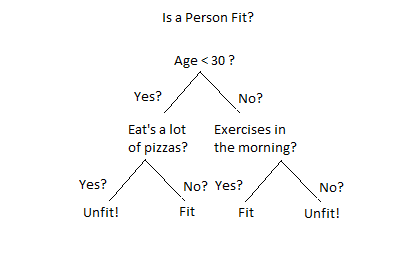
\includegraphics[width=0.45\linewidth]{figures/Decision-Trees.png}
 	\caption{}
 	\label{fig:Trees}
 \end{figure} 	
 
 we asked several questions to determine an algorithm that will tell us if a person is fit or not based on their replies. The questions are not necessarily the optimal ones, but this illustrates the general methods:  we split data points into subsets based on the values on certain features. The order in which we choose the features give us different algorithms. You can find an algorithm in the notebook ``Decision Trees'' where we aim to find the best features to consider in the decision.


 \subsection{KNN}
 In K-Nearest-Neighbors, we make a prediction or classify an element by  only analyzing  a neighborhood of the element an assigning to it a function of this neighborhood values, for example  given a new point $x$ and the closest $k$ points to $x$, you can assign to $x$ the average of $x$'s neighbors values.
 $K$ stands for how many points nearby do you consider to make your choice. The results depend on a good selection of the parameter $K$.  If the boundary is a concern,  Kernel Regression assigns different weights to the nearby points so that points that are closer matter most. Locally weighted polynomial  regression is a local version of polynomial regression where we find the best line or curve that approximate the local nbh.
  The possibility to write a model that deals with the local picture is important in applications, in fig:\ref{fig:knn} we see examples locally weighted polynomial regression.
 
 \begin{figure}[h!]
 	\centering
 	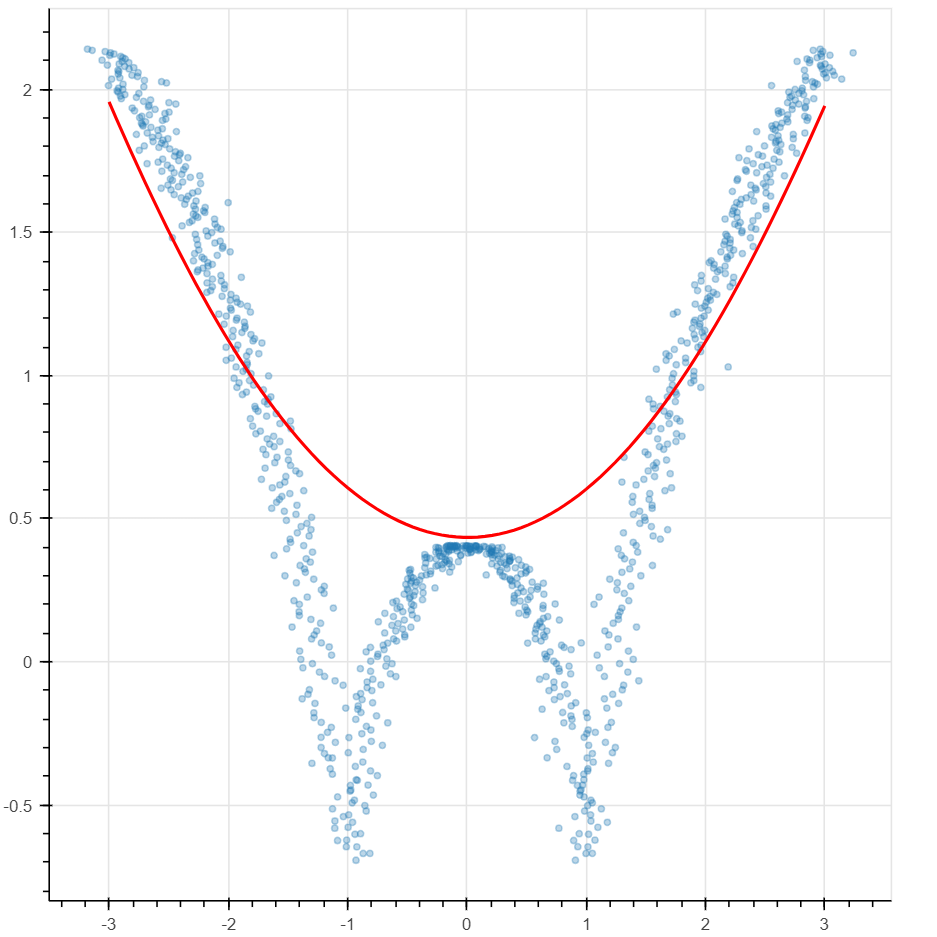
\includegraphics[width=0.25\linewidth]{figures/bokeh_plot0.png}
 	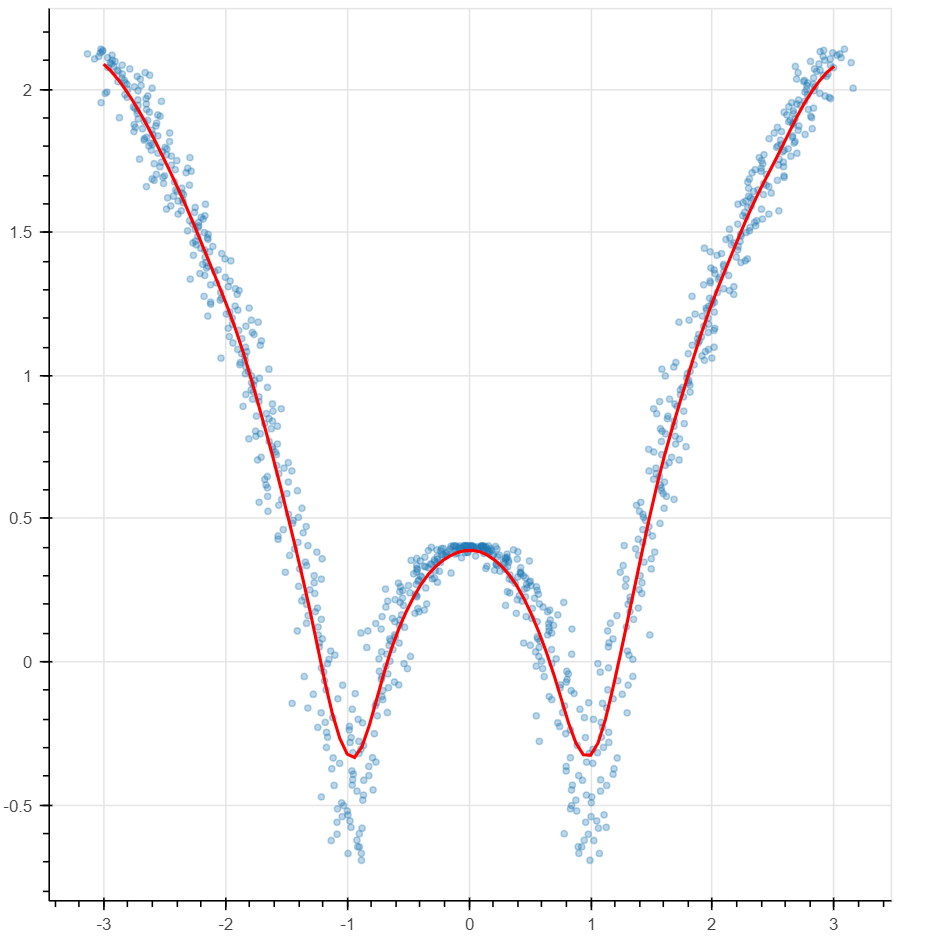
\includegraphics[width=0.25\linewidth]{figures/bokeh_plot.png}
 	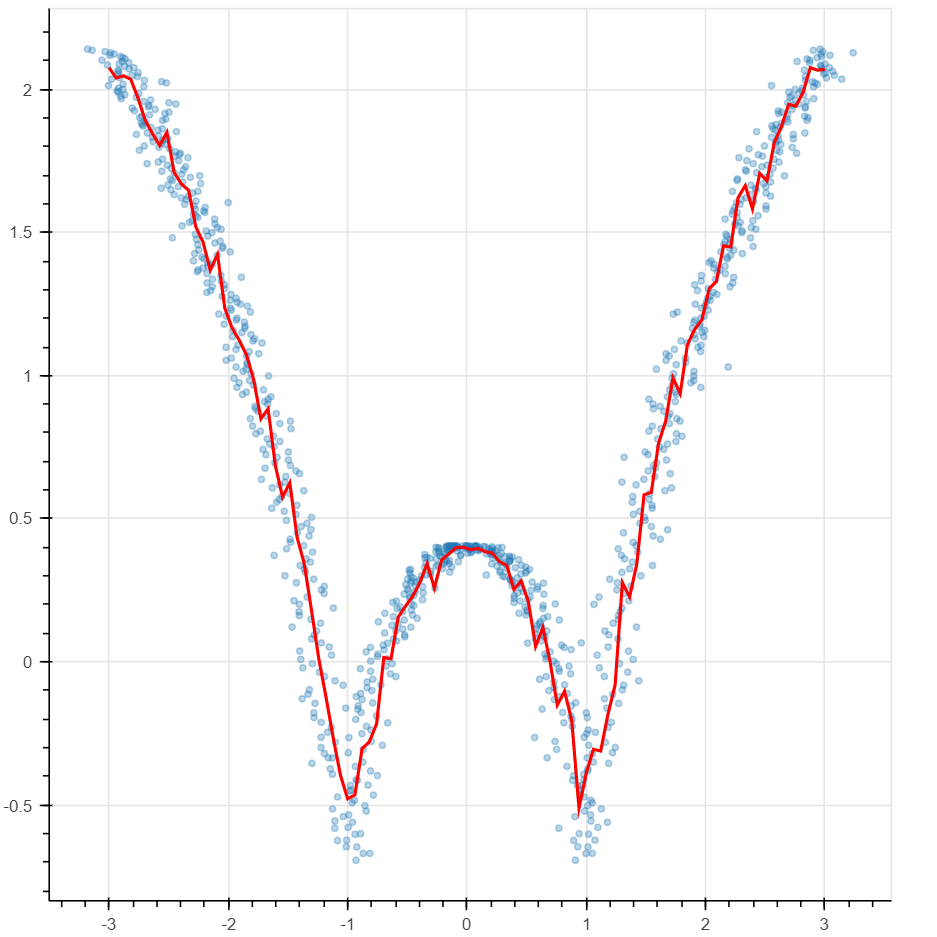
\includegraphics[width=0.25\linewidth]{figures/bokeh_plot1.png}
 	\caption{}
 	\label{fig:knn}
 \end{figure} 	
  
This should remind us of  typical diagrams in phase transition as the Mexican hat \ref{fig:face}.
 \begin{figure}[h!]
	\centering
	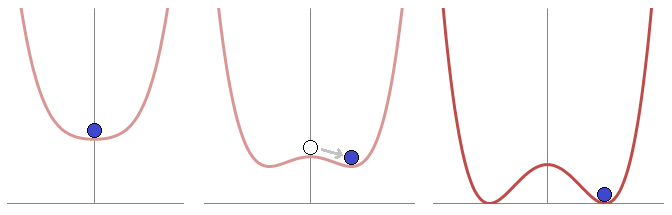
\includegraphics[width=0.45\linewidth]{figures/image.png}
	\caption{The 3d mexican hat potential.} 
	\label{fig:face}
\end{figure} 	




 \subsection{Non Negative Tensor Factorization}
 
We consider data in form of a matrix. For example, given a vocabulary with  m  words, and  n  documents,  $V_{ik}$ is  the number of times the  $i$ -word in the dictionary appears on the  $k$  document.
A database of gray-scale images of a fixed size can also be described by a matrix $V$.  We relabel the pixels in an image form $1$ to $ m$, and assume the  database has $n$ images. The value of the $V_{ik}$ is the intensity of the $i$-pixel in the $k$ image. 

Non negative matrix factorization is a process to find two matrices with non negative entries $W,H$ so that $V\sim W\times H$. It turns out that the columns of $H$ can be understood as a basis whose linear combination approximates the columns of $V$. $W$ give us the coefficients so that a juxtaposition of the columns of  $H$ can recover the initial data. Columns of $H$ have been recognized as eigen images \cite{Lee1999}.  
 
 

Imagine that for every patient you have a matrix of diagnosis and medications. We can put the column of medications and the rows of diagnosis. So the entries will be mostly zeroes, except when the patient was diagnosed with the $i$-sickness and received the $k$-medication. If we stack this matrices on each other, then we have a 3-dimensional matrix or a vector where we consider the third dimension given by the patients. There is a higher dimensional version of tensor factorization  where we substitute  matrices by tensors (higher dimensional matrices). 
 
The main yoga was that the non negativity constrain allow us to recover the initial object from juxtaposition of it's parts. When we  replaced matrices by tensors we substitute the factorization into matrix multiplication by tensor decomposition into rank one tensors. 
 
 
In Medicine, Tensor decomposition into rank one tensor shows concurring diagnosis and medications, this process is known as phenotyping\cite{Ho}.  The study of tensors (phenotypes) using machine learning lead to the discovering of 3 distinct groups of Hearth Failure with preserved Ejection Fractions (HFpEF), those groups 'differed markedly in clinical characteristics, cardiac structure / function, invasive hemodynamics, and outcomes' \cite{Shah2015}.
 
 

		%should we include reaction networks??????
			
		
\subsection{Which method to use?}
Classification Trees are used when you have Discrete output. It's a Supervised Learning algorithm (ID3, C4.5). We use it when we have a finite number of classification categories and the data can be represented as vectors.
It has the advantage that we can understand how the classifier makes its choices.


Genetic Algorithms are used for discrete parameter optimization. It's good for combinatorial problems.
They are slow and  challenging to code as it is not trivial to  find the right representations, the fitness function, etc.




Nearest Neighbor, KNN, Kernel regression, and Locally weighted (linear) regression

The algorithms are easy to understand, and are Local in nature, training data that is localized around the query contribute more to the prediction value.
They require retaining all training examples in memory, they are slow to evaluate a new query. Evaluation time grows with the dataset size.

Self Organizing Maps are unsupervised learning algorithm used for clustering and dimension reduction.


Support Vector Machines are used for Classification.
They scale well to hight dimensional data.
By designing carefully the kernels it can be used on data not on vector form as graphs, sequences, relational data, etc. It needs the parameters kernel, and how much 'slack' is allowed.


Artificial Neural Networks are a hierachical (or deep) method. While it is very popular, most problems can be solved with simpler machine learning methods\cite{Gron}. Neural networks can represent logic functions (and, or, nand) and therefore are generalizable to any complicated computer function (given enough blocks). We use CNN to work with images, with CNN it's recommended to do data-augmentation. We use RNN to analyze time series, for example in Natural Language Processing.
It is still not clear what architecture\cite{Lin2017} to use for a particular problem,   the deepness of the ANN, etc. In that direction the suggested architecture to try when dealing with images will be dilated residual networks\cite{DRN}. As for other data types, the current status of the theory says to find on research papers the architectures that other people have tried for similar problems.


Bayes methods. In this methods parameters and data are random variables. It learns the full distribution, everything about the data. With a well chosen prior, bias and over fitting is often of little concern. In practice it is computationally intractable. Must use approximation methods such as variational inference and Monte Carlo techniques.

 Monte Carlo methods began as a way to estimate high dimensional integrals using probabilistic methods. "Typically, Markov chain Monte Carlo sampling can only approximate the target distribution, as there is always some residual effect of the starting position."\cite{wmcmc}.

Non negative matrix factorization can be use for topic modeling and finding eigenfaces. It has the advantage of having meaningful outputs\cite{Lee1999}. Non negative tensor factorization is a fuzzy clustering algorithm, it is possible to use it with   Sparse data\cite{Ho2014a}. The input data should be in tensor form.

Generative Adversarial Networks and Variational Autoencoders are very popular generative methods. GAN's are difficult to train and after each iteration the optimization problem changes, so it is also hard to predict the time required for the algorithms to converge. 


\section{Experimental topics}We also described topics whose application to science may take some time but are definitely promising: an introduction to quantum computing with DWave, IBM Q and qiskit as well a notebook on reaction networks.
%Perhaps to add a diagram that helps with the classification
	
	%%%%%%%%%%%%%%%%%%%%%%%%%%%%%%%%%%%%
	% Begin Appendix Bibliography Document %%%%%%%%%%%%%%%%%%%%%
	%%%%%%%%%%%%%%%%%%%%%%%%%%%%%%%%%%%%
	
	\bibliographystyle{unsrt}
	\bibliography{ML}
	
	
\end{document}


	
Advantages of Genetic Algorithms. They does not require any derivative information (which may not be available for many real-world problems). They have very good parallel capabilities. They always give an answer to the problem, which gets better over the time.
Useful when the search space is very large and there are a large number of parameters involved.

Limitations. GAs are not suited for all problems, especially problems which are simple and for which derivative information is available. Probably we don't get the global optimum solution. Fitness value is calculated repeatedly which might be computationally expensive for some problems.
Being stochastic, there are no guarantees on the optimality or the quality of the solution.
If not implemented properly, the GA may not converge to the optimal solution.


Advantages of decision trees:
They are simple to understand, they can handle both numerical and categorical data, they are relatively little data preparation needed, the mechanism for the model can be easily extracted and understood, they are robust against co-linearity.

Disadvantages: Accuracy, they tend to overfit, and the locality of optimization.

In this notebook we deal with  memory based algorithms, 
they are all easy to adapt to new training samples, so there is no need to retrain them. They 
can handle complex decision boundaries and functions by considering the query instance when deciding how to generalize.
The cons are that they require retaining all training examples in memory, so it is slow to evaluate a new query and the evaluation time grows with the dataset size.



